\section{Experiments}
\label{section:experiments}

%song dataset
\subsection{Song Dataset}
Song dataset consisting 2300 sinhala songs were used in the registration step of the experiment. These 2300 sinhala songs were retrieved from
\gls{osca} of Sri Lanka which works as the governing organization to ensure intellectual property rights of music in Sri Lanka. 

%query audio samples
\subsection{Query Audio Samples}
Variable sized 844 query audio clips were used for the experiment to evaluate the performance of this method
against different durations. 519 of the above mentioned audio clips had songs which are in the database while 325 audio clips didn't have songs from 
the database. Hence for each test case, sample size was 844 query audio clips with 0.61492 prevalence.    

%test cases
\subsection{Test Cases}
Test cases were created by doing audio distortions to the query audio samples. Performance of the method was evaluated for three main audio distortions
which are tempo alteration, pitch alteration and both pitch and tempo alteration. Both increased and decreased alterations are considered for three different
levels of alterations which are 10\% alteration, 20\% alteration and 50\% alteration. Hence there are 3 audio distortions, 2 audio distortion directions and
3 audio alteration levels, 18 (\(3 \times 2 \times 3\)) test cases were generated to evaluate the performance. 

%test results
\subsection{Test Results}

The proposed method has an exact way to identify whether a query audio clip has a matching registered song or not. Therefore this method can be considered as
a classifier. A classifier can be evaluated by the confusion matrix generated for a given sample. \gls{tp}, \gls{fp}, \gls{tn} and \gls{fn} were calculated
for each test case. Then accuracy and \gls{fp} rate was calculated for each test case. Reducing \gls{fp} rate is significant as much as increasing the accuracy
given that this method mainly focuses on identifying music on radio broadcasts. Accuracy and \gls{fp} rate can be calculated from the formulas given below. 

\begin{align*}
    \text{Accuracy} &= \frac{TP+TN}{TP+TN+FP+FN}\\
    \\
    \text{FP Rate} &= \frac{FP}{FP+TN}\\
\end{align*}

Keypoint ratio based threshold is proposed as the threshold measure in this method. Two experiments were done, one with keypoint count as threshold measure and the
other with keypoint ratio as threshold measure to validate the claim of keypoint ratio is better threshold measure. 

\subsubsection{Using Keypoint Count as Threshold}

Average accuracies for different threshold values are illustrated as shown in Figure \ref{fig:threshold_old} to identify the optimal threshold value to use. Since
the visualization clearly indicates a global peak value which is keypoint count of 69, that value can be used as the threshold value. This threshold value of 69 is
used in this experiment. 
\vspace{12pt}

Results of the experiment using keypoint count as the threshold measure are presented in Table \ref{tab:test_results_keypoint}. There is no clear
change between accuracies of pitch changes and tempo changes when using keypoint count as the threshold measure. Pitch changes and tempo changes
up to 20\% alteration can be identified with 92\%-98\% accuracy. 


\begin{figure}[h]
    \centering
    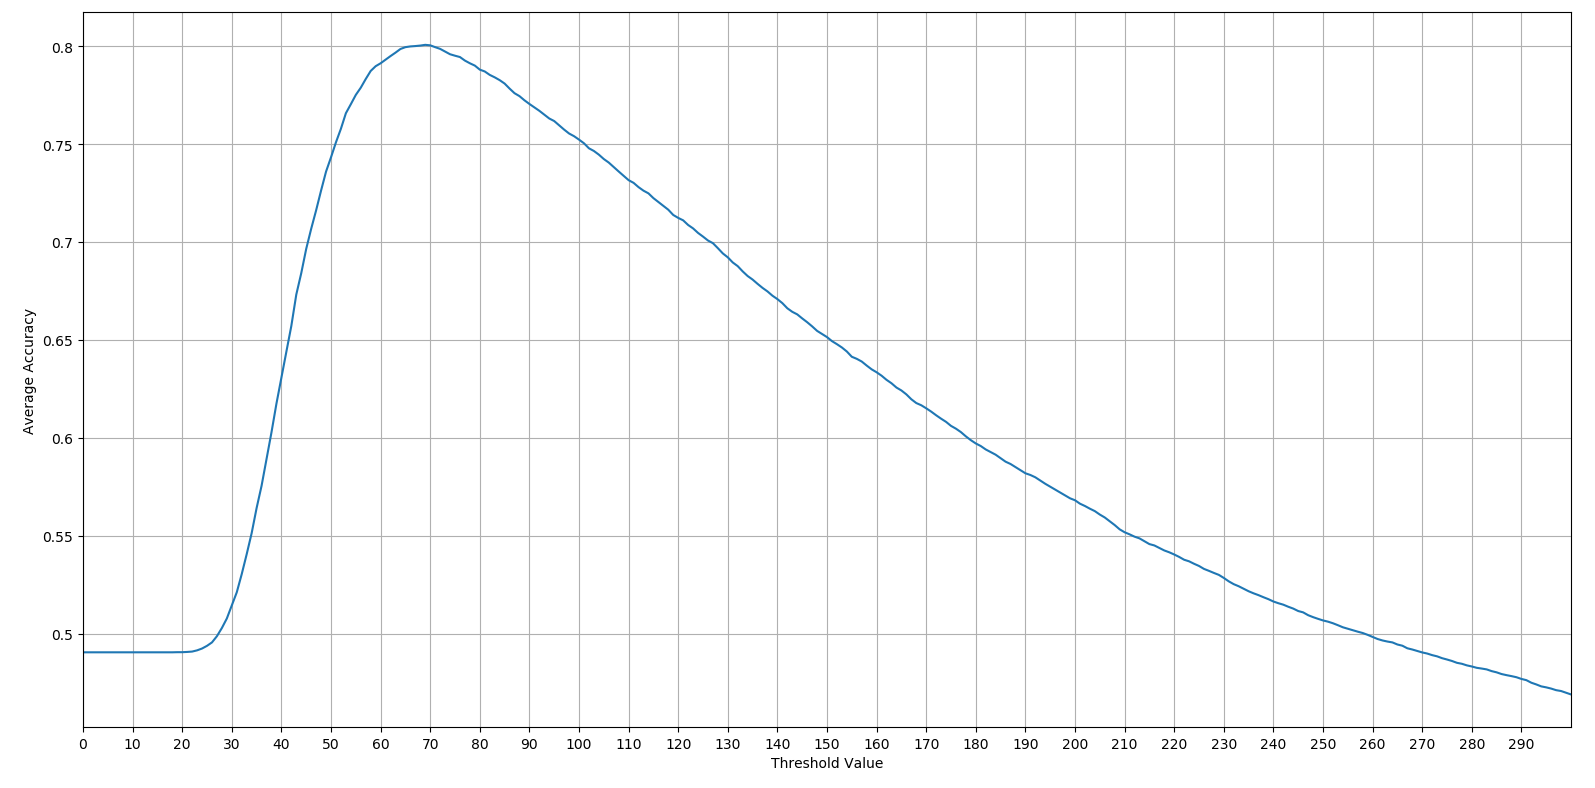
\includegraphics[scale=0.21]{images/threshold_adjusting_old.png}
    \caption{Average Accuracy Values for Different Threshold Values (Keypoint Count)}
    \label{fig:threshold_old}
  \end{figure}
  


\begin{table}[H]
    \begin{tabular}{|L|r|r|r|r|r|r|}
        \hline
        \vspace{5pt}\textbf{Test Case}\vspace{5pt}                  & \textbf{TP}   & \textbf{FP} & \textbf{TN} & \textbf{FN} & \textbf{Accuracy} & \textbf{FP Rate} \\ \hline
        Tempo Increase 10\%                & 509         & 19          & 306         & 10          & 0.96564           & 0.05846          \\ \hline
        Tempo Increase 20\%                & 509         & 18          & 307         & 10          & 0.96682           & 0.05538          \\ \hline
        Tempo Increase 50\%                & 497         & 10          & 315         & 22          & 0.96209           & 0.03077          \\ \hline
        Tempo Decrease 10\%                & 515         & 16          & 309         & 4           & 0.97630           & 0.04923          \\ \hline
        Tempo Decrease 20\%                & 516         & 19          & 306         & 3           & 0.97393           & 0.05846          \\ \hline
        Tempo Decrease 50\%                & 517         & 22          & 303         & 2           & 0.97156           & 0.06769          \\ \hline
        Pitch Increase 10\%                & 514         & 21          & 304         & 5           & 0.96919           & 0.06462          \\ \hline
        Pitch Increase 20\%                & 513         & 11          & 314         & 6           & 0.97986           & 0.03385          \\ \hline
        Pitch Increase 50\%                & 7           & 27          & 298         & 512         & 0.36137           & 0.08308          \\ \hline
        Pitch Decrease 10\%                & 511         & 11          & 314         & 8           & 0.97749           & 0.03385          \\ \hline
        Pitch Decrease 20\%                & 463         & 4           & 321         & 56          & 0.92891           & 0.01231          \\ \hline
        Pitch Decrease 50\%                & 0           & 0           & 325         & 519         & 0.38507           & 0.00000          \\ \hline
        Tempo \& Pitch Increase 10\%       & 414         & 11          & 314         & 105         & 0.86256           & 0.03385          \\ \hline
        Tempo \& Pitch Increase 20\%       & 339         & 18          & 307         & 180         & 0.76540           & 0.05538          \\ \hline
        Tempo \& Pitch Increase 50\%       & 0           & 26          & 299         & 519         & 0.35427           & 0.08000          \\ \hline
        Tempo \& Pitch Decrease 10\%       & 373         & 5           & 320         & 146         & 0.82109           & 0.01538          \\ \hline
        Tempo \& Pitch Decrease 20\%       & 226         & 2           & 323         & 293         & 0.65047           & 0.00615          \\ \hline
        Tempo \& Pitch Decrease 50\%       & 0           & 0           & 325         & 519         & 0.38507           & 0.00000          \\ \hline
    \end{tabular}
    \vspace{12pt}
    \caption{Experiment results using keypoint count as threshold}
    \label{tab:test_results_keypoint}
\end{table}


\subsubsection{Using Keypoint Ratio as Threshold}

Average accuracies for different threshold values are illustrated as shown in Figure \ref{fig:threshold_new} to identify the optimal threshold value to use. Since
the visualization clearly indicates a global peak value which is keypoint count of 0.0403, that value can be used as the threshold value. This threshold value of 
0.0403 is used in this experiment. 
\vspace{12pt}

Results of the experiment using keypoint ratio as the threshold measure presented in Table \ref{tab:test_results_keypoint_ratio}. It can be observed that accuracies
have increased considerably compared to results of the experiment which uses keypoint count as the threshold measure which validates the claim of taking keypoint ratio as
a better threshold measure. Pitch changes and tempo changes up to 20\% alteration can be identified with 95\%-99\% accuracy.

\begin{figure}[h]
    \centering
    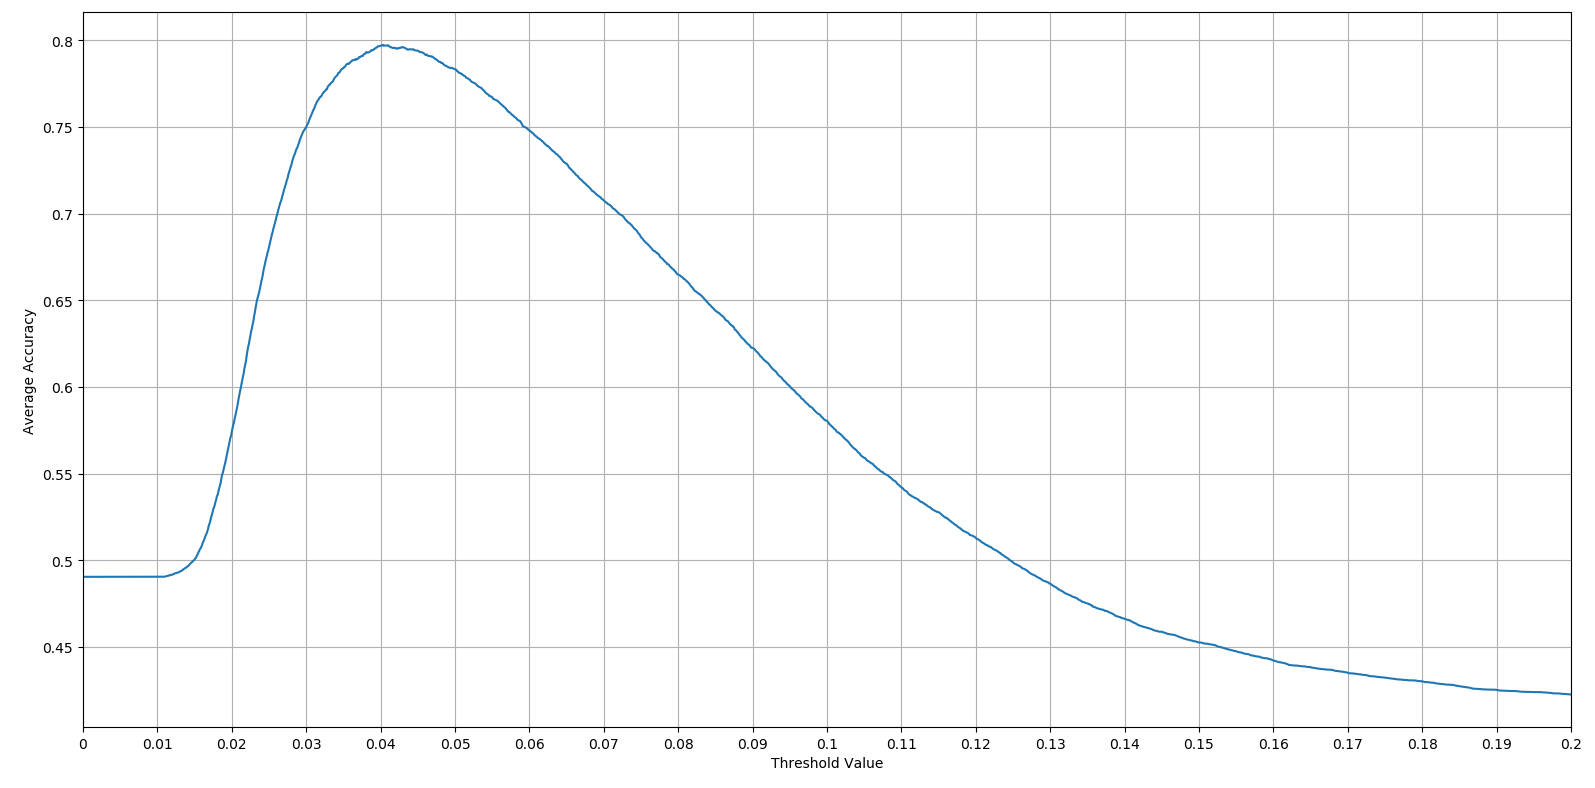
\includegraphics[scale=0.21]{images/threshold_adjusting.png}
    \caption{Average Accuracy Values for Different Threshold Values (Keypoint Ratio)}
    \label{fig:threshold_new}
  \end{figure}

\begin{table}[H]
    \begin{tabular}{|L|r|r|r|r|r|r|}
        \hline
        \vspace{5pt}\textbf{Test Case}\vspace{5pt}                & \textbf{TP}   & \textbf{FP} & \textbf{TN} & \textbf{FN} & \textbf{Accuracy} & \textbf{FP Rate} \\ \hline
        Tempo Increase 10\%                & 512         & 13          & 312         & 7           & 0.97630           & 0.04000          \\ \hline
        Tempo Increase 20\%                & 508         & 10          & 315         & 11          & 0.97512           & 0.03077          \\ \hline
        Tempo Increase 50\%                & 501         & 9           & 316         & 18          & 0.96801           & 0.02769          \\ \hline
        Tempo Decrease 10\%                & 515         & 11          & 314         & 4           & 0.98223           & 0.03385          \\ \hline
        Tempo Decrease 20\%                & 519         & 10          & 315         & 0           & 0.98815           & 0.03077          \\ \hline
        Tempo Decrease 50\%                & 519         & 9           & 316         & 0           & 0.98934           & 0.02769          \\ \hline
        Pitch Increase 10\%                & 519         & 9           & 316         & 0           & 0.98934           & 0.02769          \\ \hline
        Pitch Increase 20\%                & 517         & 9           & 316         & 2           & 0.98697           & 0.02769          \\ \hline
        Pitch Increase 50\%                & 0           & 4           & 321         & 519         & 0.38033           & 0.01231          \\ \hline
        Pitch Decrease 10\%                & 516         & 16          & 309         & 3           & 0.97749           & 0.04923          \\ \hline
        Pitch Decrease 20\%                & 503         & 25          & 300         & 16          & 0.95142           & 0.07692          \\ \hline
        Pitch Decrease 50\%                & 23          & 160         & 165         & 496         & 0.22275           & 0.49231          \\ \hline
        Tempo  \& Pitch Increase 10\%      & 413         & 11          & 314         & 106         & 0.86137           & 0.03385          \\ \hline
        Tempo  \& Pitch Increase 20\% & 287         & 17          & 308         & 232         & 0.70498           & 0.05231          \\ \hline
        Tempo  \& Pitch Increase 50\% & 0           & 7           & 318         & 519         & 0.37678           & 0.02154          \\ \hline
        Tempo  \& Pitch Decrease 10\% & 432         & 28          & 297         & 87          & 0.86374           & 0.08615          \\ \hline
        Tempo  \& Pitch Decrease 20\% & 346         & 34          & 291         & 173         & 0.75474           & 0.10462          \\ \hline
        Tempo  \& Pitch Decrease 50\% & 6           & 154         & 171         & 513         & 0.20972           & 0.47385          \\ \hline
    \end{tabular}
    \vspace{12pt}
\caption{Experiment results using keypoint ratio as threshold}
\label{tab:test_results_keypoint_ratio}
\end{table}


\subsection{Evaluation}

Final results of the experiment with keypoint ratio as the threshold measure performs significantly better
than the keypoint count threshold measure. Hence, it can be concluded that keypoint ratio is a better
threshold measure than keypoint count.
\vspace{12pt}

There is a sudden drop of accuracies between 20\% and 50\% pitch changes. This sudden drop happens when shifting
up or down on the frequency axis making spectrogram local patterns to be compressed or expanded which makes the pattern
to get unidentified as shown in Figure \ref{fig:spectrogram_down}.


\begin{figure}[h]
    \centering
    \includegraphics[scale=0.5]{images/spectrogram_down.png}
    \caption{Generated colour image of a spectrogram (50\% pitch decrease)}
    \label{fig:spectrogram_down}
  \end{figure}